% \iffalse meta-comment
%
% Copyright (c) 2026- Jesse Straat
% 
% This work may be distributed and/or modified under the
% conditions of the LaTeX Project Public License, either version 1.3
% of this license or (at your option) any later version.
% The latest version of this license is in
%   https://www.latex-project.org/lppl.txt
% and version 1.3c or later is part of all distributions of LaTeX
% version 2008 or later.
%
% This work has the LPPL maintenance status `maintained'.
% 
% The Current Maintainer of this work is Jesse Straat.
%
% This work consists of the main file brandstyler.dtx
% and the derived files
%      brandstyler.sty, brandstyler.pdf, brandstyler.ins
%
% Unpacking:
% (a) If brandstyler.ins is present:
%		pdflatex brandstyler.ins
% (b) If brandstyler.ins is absent:
%		pdflatex brandstyler.dtx
%
% Documentation:
% 	    pdflatex brandstyler.dtx
%       makeindex -s gind.ist -o brandstyler.ind brandstyler.idx
%       makeindex -s gglo.ist -o brandstyler.gls brandstyler.glo
%       pdflatex brandstyler.dtx
%
%<*ignore>
\iffalse
%</ignore>
%
%<*readme>
# `brandstyler`

`brandstyler` automatically adapts the
style of a LaTeX document to that of a specific organisation.
It is also compatible with `beamer`, able to change
the style of many beamerthemes.

# Installation
Run the following in the command line:
1. If brandstyler.ins is present:
    `pdflatex brandstyler.ins`
2. If brandstyler.ins is absent:
    `pdflatex brandstyler.dtx`

Move `.sty` and `.cls` files to a folder that TeX can find.

# Documentation
Run the following in the command line:
```
pdflatex brandstyler.dtx
makeindex -s gind.ist -o brandstyler.ind brandstyler.idx
makeindex -s gglo.ist -o brandstyler.gls brandstyler.glo
pdflatex brandstyler.dtx
```
This automatically unpacks the package, as well.


If you are looking for comments or documentation, you won't find
any in the source. These packages make use of literate programming, which means
that the documentation is given in the form of a pdf file. You can
probably find brandstyler.pdf in this folder, by running "texdoc --view brandstyler"
in the command line, or Googling
"[your distribution] how to find package documentation".
If you're using MiKTeX, open MiKTeX console, go to
"Documentation" and look for "brandstyler".

# Contributing
Contributions of custom brand styles are highly encouraged.
Please create a pull request on our GitHub repository at
https://github.com/JesseStraat/brandstyler. Make sure to follow
the following guidelines:
1. Brand style files should follow the same structure
as the ones supplied in this package.
2. The file should be implemented and documented in
`brandstyler.dtx`. Don't forget to update the list of files.
3. Come up with a sensible, unique identifier. For example,
Utrecht University was named `uu-nl` instead of `uu` to discern
it from Uppsala Universitet (which should be named
`uu-se`). For country abbreviations, make sure to follow
[ISO 3166-1 alpha-2](https://en.wikipedia.org/wiki/List_of_ISO_3166_country_codes)
standards.
4. If possible, use freely available or open source fonts.
5. Never include logos; they are protected by copyright, and
hence cannot be part of this open source project.

If you don't have the technical knowledge to make a brand
style, feel free to open an issue on GitHub requesting one. Please include
a link to an official style guide.

---

&copy; 2026- Jesse Straat

License: [LPPL1.3c](https://www.latex-project.org/lppl.txt)

[GitHub Repository](https://github.com/JesseStraat/brandstyler)

%</readme>
%
%<*ignore>
\fi
\def\plainTeXstring{plain}
\ifx\fmtname\plainTeXstring\else
  \expandafter\begingroup
\fi
%</ignore>
%
%<*install>
\input docstrip.tex
\Msg{************************************************************************}
\Msg{* Installation}
\Msg{* Package: brandstyler 2026/06/24 v1.0}
\Msg{************************************************************************}

\keepsilent
\askforoverwritefalse

\preamble

Copyright (c) 2026- Jesse Straat

This work may be distributed and/or modified under the
conditions of the LaTeX Project Public License, either version 1.3
of this license or (at your option) any later version.
The latest version of this license is in
  https://www.latex-project.org/lppl.txt
and version 1.3c or later is part of all distributions of LaTeX
version 2008 or later.

This work has the LPPL maintenance status `maintained'.

The current maintainer of this work is Jesse Straat.

This work consists of the main file brandstyler.dtx
and the derived files
    brandstyler.sty, brandstyler.pdf, brandstyler.ins, brandstyler-ru-nl.sty,
    brandstyler-uu-nl.sty, brandstyler-vuamst.sty

If you are looking for comments or documentation, you won't find
any in the source. These packages make use of literate programming, which means
that the documentation is given in the form of a pdf file. You can
probably find brandstyler.pdf in this folder, by running "texdoc --view brandstyler"
in the command line, or Googling
"[your distribution] how to find package documentation".
If you're using MiKTeX, open MiKTeX console, go to
"Documentation" and look for "brandstyler".

\endpreamble

\usedir{tex/latex/brandstyler}
\generate{
    \file{brandstyler.sty}{\from{\jobname.dtx}{brandstyler}}
    \file{brandstyler-ru-nl.sty}{\from{\jobname.dtx}{ru-nl}}
    \file{brandstyler-uu-nl.sty}{\from{\jobname.dtx}{uu-nl}}
    \file{brandstyler-vuamst.sty}{\from{\jobname.dtx}{vuamst}}
}

\obeyspaces
\Msg{************************************************************************}
\Msg{*}
\Msg{* To finish the installation you have to move the following}
\Msg{* files into a directory searched by TeX:}
\Msg{*}
\Msg{*    brandstyler.sty}
\Msg{*    any brandstyler sty file you want to use}
\Msg{*}
\Msg{* To produce the documentation run the file `brandstyler.dtx'}
\Msg{* through LaTeX.}
\Msg{*}
\Msg{* Happy TeXing!}
\Msg{*}
\Msg{************************************************************************}

%</install>
%<install>\endbatchfile
%
%<*ignore>
\usedir{source/latex/brandstyler}
\generate{
    \file{\jobname.ins}{\from{\jobname.dtx}{install}}
}

\nopreamble\nopostamble
\usedir{doc/latex/brandstyler}
\generate{
    \file{README.md}{\from{\jobname.dtx}{readme}}
}

\ifx\fmtname\plainTeXstring
  \expandafter\endbatchfile
\else
  \expandafter\endgroup
\fi
%</ignore>

%<*driver>
\NeedsTeXFormat{LaTeX2e}[2020/10/01]
\documentclass{ltxdoc}
\usepackage{\jobname}
\usepackage[english]{babel}
\usepackage[final,
hyperindex=false,
colorlinks,
]{hyperref}
\usepackage{hologo}
\usepackage{graphicx}
\usepackage{tabularx}
\renewcommand\tabularxcolumn[1]{m{#1}}
\usepackage{ltablex}
\newcommand{\ColorName}[2]{%
    \raisebox{0.25em}{%
        \colorbox[RGB]{#2}{%
            \phantom{\rule{0.8em}{0em}}%
        }%
    }
    \texttt{\detokenize{#1}}%
}
\EnableCrossrefs
\CodelineIndex
\RecordChanges
\begin{document}
  \DocInput{\jobname.dtx}
\end{document}
%</driver>
% \fi
%
% \GetFileInfo{\jobname.sty}
%
% \DoNotIndex{\begin,\end,\@ifclassloaded,\csname,\def,\definecolor,\else,\endcsname}
% \DoNotIndex{\familydefault,\fi,\ifcsname,\IfFileExists,\IfFontExistsTF,\ifpdftex}
% \DoNotIndex{\mode,\newcommand,\PackageError,\PackageWarning,\ProvidesPackage}
% \DoNotIndex{\renewcommand,\RequirePackage,\setbeamercolor,\sfdefault,\usepackage}
%
% \title{^^A
%     brandstyler\thanks{^^A
%         Version \fileversion, last revised \filedate.^^A
%     }^^A
% }^^A
% \author{^^A
% 	Jesse Straat^^A
% }
% \date{\filedate}
%
% \maketitle
%
% \begin{abstract}
%     \noindent \textsf{brandstyler} automatically adapts the
%    style of a \LaTeX{} document to that of a specific organisation.
%    It is also compatible with \textsf{beamer}, able to change
%    the style of many beamerthemes.
% \end{abstract}
%
% \tableofcontents
%
% \changes{v1.0}{2026/06/24}{First release}
%
%
%
%\StopEventually{^^A
%  \clearpage
%  \PrintChanges
%  \PrintIndex
%}
%
%
%
%
% \section{Documentation}
% This is the documentation to \textsf{brandstyler}; a package
% that automatically adapts
% the branding/style of organisations to your \LaTeX{} document.
% This is done mainly by loading the organisation's fonts and
% defining some colours.\par
% In the case of \textsf{beamer} presentations (and posters),
% \textsf{brandstyler} also automatically implements the organisation's
% colours into the presentation. The colours change best with the
% \textsf{whale} colortheme or similar.
%^^A
% \subsection{Usage}
% To use this package, use |\usepackage{brandstyler}|. Then, load
% your organisation's style using |\brandstyle{ORGANISATION}|. Make
% sure to do this after loading other style packages, such as a
% beamertheme, to make sure nothing is overwritten.\par
% An example of implementation in an article is given below.
% \begin{verbatim}
% \documentclass{article}
% \usepackage{brandstyler}
% \brandstyle{vuamst}
% 
% \begin{document}
%     Lorem Ipsum.
% \end{document}
% \end{verbatim}\par
% We also provide an implementation in beamer.
% \begin{verbatim}
% \documentclass{beamer}
% \usetheme{Frankfurt}
% \usepackage{brandstyler}
% \brandstyle{vuamst}
% 
% \begin{document}
% \begin{frame}{Foo Theory}
%     \begin{theorem}{Baz Theorem}
%       Lorem Ipsum.
%     \end{theorem}
% \end{frame}
% \end{document}
% \end{verbatim}\par
% As part of importing the style, some fonts are imported. If the
% correct font is not found on your computer, \textsf{brandstyler} will
% throw a warning informing you of that fact.
%^^A
% \clearpage
% \subsection{List of \textsf{brandstyler} files}\label{sec:filelist}
% The following brand styles are automatically part
% of this package. Each font is typeset in their font type (i.e.,
% \textrm{roman}, \textsf{sans serif} and \texttt{typewriter}).
% Furthermore, the font that is the default is boldened.
% \begin{tabularx}{\textwidth}{| m{0.15\textwidth} | m{0.15\textwidth} | m{0.2\textwidth} | X |}\hline
% \textsf{brandstyle} & Organisation & Fonts & Colour scheme\\\hline
% ^^A
% \textsf{ru-nl} & Radboud University & \textbf{\textsf{Open Sans}} &
% \ColorName{RUred-impact}{227,000,011}\newline
% \ColorName{RUpoppy}{255,066,075}\newline
% \ColorName{RUlady-bug}{190,049,026}\newline
% \ColorName{RUberry}{143,032,017}\newline
% \ColorName{RUmaroon}{115,014,004}\newline
% \ColorName{RUmahogany}{074,000,004}\newline
% \ColorName{RUgray}{121,119,119}\newline
% \ColorName{RUorange}{207,082,008}\newline
% \ColorName{RUblue}{000,138,203}\newline
% \ColorName{RUpetrol}{000,143,137}\newline
% \ColorName{RUgreen}{074,169,067}\newline
% \ColorName{RUyellow}{204,175,000}\\\hline
% ^^A
% \textsf{uu-nl} & Utrecht University & \textbf{Merriweather}\newline\textsf{Open Sans} &
% \ColorName{UUyellow}{255,205,000}\newline
% \ColorName{UUred}{192,010,053}\\\hline
% ^^A
% \textsf{vuamst} & Vrije Universiteit Amsterdam & \textbf{\textsf{Roboto}} &
% \ColorName{VUblue_primary}{000,119,179}\newline
% \ColorName{VUblue_secondary}{093,173,208}\newline
% \ColorName{VUblue_tertiary}{212,239,250}\newline
% \ColorName{VUorange_primary}{204,065,000}\newline
% \ColorName{VUorange_secondary}{232,105,045}\newline
% \ColorName{VUorange_tertiary}{252,211,182}\newline
% \ColorName{VUgreen_primary}{000,128,083}\newline
% \ColorName{VUgreen_secondary}{079,175,072}\newline
% \ColorName{VUgreen_tertiary}{235,240,198}\newline
% \ColorName{VUpurple_primary}{059,033,113}\newline
% \ColorName{VUpurple_secondary}{142,077,164}\newline
% \ColorName{VUpurple_tertiary}{221,198,238}\\\hline
% \end{tabularx}
%^^A
% \subsection{Example of an \textsf{brandstyler} file}\label{sec:brandstylerexample}
% Below is an example of a file that can be used with \textsf{brandstyler}.
% All \textsf{brandstyler} files should follow the naming scheme of
% |brandstyler-NAME.sty|. As an example, we will implement the brand guide
% of the \href{https://www.gov.uk/government/publications/govuk-brand-guidelines}{United Kingdom government}.
% We will name the file |brandstyler-ukgov.sty|. It can be used by running the
% macro |\brandstyle{ukgov}| in your \LaTeX{} file. An example of this style can be
% found in \autoref{fig:ukgovexample}.
% \begin{verbatim}
% 1. \definecolor{UKprimary-blue}{RGB}{029,112,184}
% 2. \definecolor{UKaccent-teal}{RGB}{000,255,224}
% 3. \definecolor{UKprimary-green}{RGB}{017,125,090}
% 4. \definecolor{UKprimary-red}{RGB}{202,053,053}
% 5. \definecolor{UKprimary-yellow}{RGB}{255,221,000}
% 6. \def\brandstyler@tfsansfont{GDS Transport}
% 7. \def\brandstyler@pdffont{\renewcommand\sfdefault{phv}}
% 8. \renewcommand{\familydefault}{\sfdefault}
% 9. \@ifclassloaded{beamer}{%
%10.     \mode<presentation>
%11.     \setbeamercolor{structure}{fg=UKprimary-blue}
%12.     \setbeamercolor{alerted text}{fg=UKprimary-red}
%13.     \setbeamercolor{example text}{fg=UKprimary-green}
%13.     \mode
%14.     <all>
%14. }{}
% \end{verbatim}
% \begin{figure}
%   \centering
%   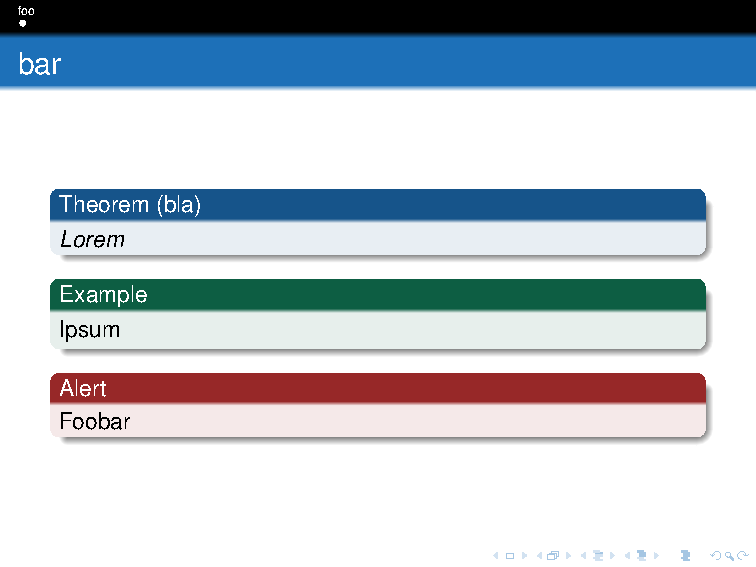
\includegraphics[width=0.6\textwidth]{ukgovtest.pdf}
%   \caption{An example of a \textsf{beamer} slide using the \textsf{Frankfurt}
%   beamer theme, \textsf{brandstyler} and the \texttt{ukgov} style as outlined in 
%   \autoref{sec:brandstylerexample}. \hologo{pdfLaTeX} was used for compilation
%   (and hence the actual font is \texttt{phv}).}\label{fig:ukgovexample}
% \end{figure}
% We will now go through this code line by line.\par
% In lines 1--5, we define all relevant colours for the style.
% Give them a recognisable name, so they can easily be used by the
% end user. Make sure not to use actual names of colours,
% like ``blue'' or ``maroon'', since they may interfere with
% those defined by \LaTeX{} itself. It's best to prepend each colour with
% a (capitalised) abbreviation of the organisation, and not use capital
% letters for the colour itself. Note that not all colours may be
% actually used by \textsf{brandstyler}; defining them here is nonetheless
% useful for users.\par
% We define the fonts in lines 6--8. The UK government only specifies a sans
% serif font, GDS Transport. We save the font to a variable using
% \DescribeMacro{\brandstyler@tfsansfont} |\brandstyler@tfsansfont|.
% A serif/Roman font can be defined in the same way using
% \DescribeMacro{\brandstyler@tfmainfont} |\brandstyler@tfmainfont|,
% and a typewriter font can be defined using
% \DescribeMacro{\brandstyler@tfmonofont} |\brandstyler@tfmonofont|.\par
% For \hologo{pdfLaTeX} users, just selecting a font won't work,
% since \hologo{pdfLaTeX} doesn't support ordinary
% font formats such as |otf| and |ttf|. Therefore, we will have to
% use a \hologo{pdfLaTeX}-compatible font, instead. We save the code used
% to load all fonts into a single variable, \DescribeMacro{\brandstyler@pdffont}
% |\brandstyler@pdffont| in line 7.\par
% Of course, \hologo{pdfLaTeX} doesn't support GDS Transport, at all.
% As an alternative, the UK government mentions using Neue Helvetica.
% Although \hologo{pdfLaTeX} doesn't support this, either, it does
% support Helvetica, under the name |phv|.\par
% If we were to use a font for which we need
% an external package, we should instead use |\usepackage{PACKAGE}| to
% load the fonts. If we also want to load a serif or typewriter font,
% we should put them all in the single variable.\par
% Since the UK government brand guide specifies only a sans serif font
% should be used, we should also tell \LaTeX{} to use it instead of the
% main serif font, in line 8.\par
% Finally, in lines 9--16, we define the behaviour of our style in Beamer. Theoretically,
% one may put any Beamer style commands in here, but we recommend to only
% change some colours around. The most important colour to change is
% the |structure| colour, which will, depending on you \textsf{beamer}
% theme, determine almost all colours on your presentation. Set this
% to whatever colour is considered primary by your organisation. If your
% organisation has an official reddish colour and greenish colour, feel
% free to also change the colours of |alerted| and |example| text, which
% usually also changes the corresponding boxes.
%^^A
% \subsection{\texorpdfstring{\textsf{beamer}}{Beamer} compatibility}
% \textsf{brandstyler} is compatible with many beamerthemes, but not all.
% To work, it is essential the theme is built on the |structure| colour.
% This is true of most themes featuring the classical ``beamer blue''
% colour scheme. Examples of such beamerthemes are \textsf{Frankfurt},
% \textsf{Berlin}, and others. However, some beamerthemes manually set the
% colour of each element, such as \textsf{CambridgeUS}, which causes an
% incompatibility.
%^^A
% \subsection{Contributing}
% Contributions of custom brand styles are highly encouraged.
% Please create a pull request on our GitHub repository at
% \url{https://github.com/JesseStraat/brandstyler}. Make sure to follow
% the following guidelines:
% \begin{enumerate}
%   \item Brand style files should follow the same structure
%   as the ones supplied in this package.
%   \item The file should be implemented and documented in
%   |brandstyler.dtx|. Don't forget to update the list of files
%   in \autoref{sec:filelist}.
%   \item Come up with a sensible, unique identifier. For example,
%   Utrecht University was named |uu-nl| instead of |uu| to discern
%   it from Uppsala Universitet (which should be named
%   |uu-se|). For country abbreviations, make sure to follow
%   \href{https://en.wikipedia.org/wiki/List_of_ISO_3166_country_codes}{ISO 3166-1 alpha-2}
%   standards.
%   \item If possible, use freely available or open source fonts.
%   \item Never include logos; they are protected by copyright, and
%   hence cannot be part of this open source project.
%   \item Supply a source where the style guide is defined. It's
%   alright (but not preferable) if the style guide is inaccessible
%   for people outside the organisation. However, in such cases, the
%   source should be a public ``lander'' which forwards to the guide,
%   so one can check it's a genuine style guide.
% \end{enumerate}
% If you don't have the technical knowledge to make a brand
% style, feel free to open an issue on GitHub requesting one. Please include
% a link to an official style guide.
%
%
%
% \clearpage
% \section{Source code}
% This section contains the source code of the library.
% It contains some explaining descriptions, allowing for
% \href{https://https://en.wikipedia.org/wiki/Literate_programming}{literate programming}.
% This is where the documentation for ``regular people'' ends.
%^^A
%^^A
%^^A
%^^A
% \setcounter{CodelineNo}{0}
%    \begin{macrocode}
%<*brandstyler>
\ProvidesPackage{brandstyler}[2026/06/24 v1.0 Brand style implementer]
\RequirePackage{iftex}
\RequirePackage{xcolor}
%    \end{macrocode}
% \begin{macro}{\brandstyle}
% Loads brand styles.
%    \begin{macrocode}
\newcommand{\brandstyle}[1]{%
    \IfFileExists{brandstyler-#1.sty}{%
%    \end{macrocode}
% The brand style file exists;
% we will import its parameters.
%    \begin{macrocode}
        \usepackage{brandstyler-#1}%
%    \end{macrocode}
% We implement the parameters in several
% commands.
%    \begin{macrocode} 
        \brandstyler@font
    }{%
        % File not found
        \PackageError{brandstyler}%
        {The brand style '#1'
        was not found.}%
        {Check for typos or create your
        own brand style.}%
    }
}
%    \end{macrocode}
% \end{macro}
% \begin{macro}{\brandstyler@font}
% The included fonts are imported. We automatically check whether
% the engine used is \hologo{pdfLaTeX}. If this is the case, we
% use a corresponding font. If not, we assume the compiler is
% \textsf{fontspec}-compatible.
%    \begin{macrocode}
\newcommand{\brandstyler@font}{%
    \ifpdftex
        \brandstyler@load@pdffont
    \else
        % Assume fontspec: use typefont
        \RequirePackage{fontspec}
        \brandstyler@load@tffont
    \fi
}
%    \end{macrocode}
% \end{macro}
% \begin{macro}{\brandstyler@load@pdffont}
% We import a \hologo{pdfLaTeX}-compatible font. Since the possible
% input of such fonts is highly variable, we just assume the input
% is a piece of code which loads the fonts.
%    \begin{macrocode}
\newcommand{\brandstyler@load@pdffont}{%
    \ifcsname brandstyler@pdffont\endcsname
        \brandstyler@pdffont
    \fi
}
%    \end{macrocode}
% \end{macro}
% \begin{macro}{\brandstyler@load@tffont}
% The engine is compatible with \textsf{fontspec}, likely either
% \hologo{LuaLaTeX} or \hologo{XeLaTeX}. The fonts are just
% typefont files (either |.otf| or |.ttf|), and can thus be loaded
% straightforwardly.
%    \begin{macrocode}
\newcommand{\brandstyler@load@tffont}{%
    \ifcsname brandstyler@tfmainfont\endcsname
        \brandstyler@existsload@tffont{\brandstyler@tfmainfont}{main}
    \fi
    \ifcsname brandstyler@tfsansfont\endcsname
        \brandstyler@existsload@tffont{\brandstyler@tfsansfont}{sans}
    \fi
    \ifcsname brandstyler@tfmonofont\endcsname
        \brandstyler@existsload@tffont{\brandstyler@tfmonofont}{mono}
    \fi
}
%    \end{macrocode}
% \end{macro}
% \begin{macro}{\brandstyler@existsload@tffont}
% This macro checks whether a typefont exists or not. If It
% does, the font is loaded. The first argument should be the name
% of the font, e.g., |Helvetica|. The second argument should be
% the type of font, i.e., |main| for \textrm{serif/Roman}, |sans| for \textsf{sans serif},
% or |mono| for \texttt{typewriter fonts}.
%    \begin{macrocode}
\newcommand{\brandstyler@existsload@tffont}[2]{%
    \IfFontExistsTF{#1}
        {\csname set#2font\endcsname{#1}}
        {
            \PackageWarning{brandstyler}{Font #1 not found. 
            Your organisation recommends its usage. 
            Please install it from the internet, you organisation
            or your LaTeX distribution.}
        }
}
%    \end{macrocode}
% \end{macro}
%    \begin{macrocode}
%</brandstyler>
%    \end{macrocode}
% From this point onwards, we will consider the implementation
% of the brand style files of various organisations.
% Wherever possible, we only use freely available
% fonts, in order to accomodate users (usually students)
% who don't have access to those fonts.
% 
% \subsection{\textsf{ru-nl}: Radboud University}
% \href{https://www.ru.nl/en/staff/services/campus-facilities-buildings/communication-and-promotion/design/corporate-identity}{Source.}\par
%    \begin{macrocode}
%<*ru-nl>
\definecolor{RUred-impact}{RGB}{227,000,011}
\definecolor{RUpoppy}{RGB}{255,066,075}
\definecolor{RUlady-bug}{RGB}{190,049,026}
\definecolor{RUberry}{RGB}{143,032,017}
\definecolor{RUmaroon}{RGB}{115,014,004}
\definecolor{RUmahogany}{RGB}{074,000,004}

\definecolor{RUgray}{RGB}{121,119,119}
\definecolor{RUorange}{RGB}{207,082,008}
\definecolor{RUblue}{RGB}{000,138,203}
\definecolor{RUpetrol}{RGB}{000,143,137}
\definecolor{RUgreen}{RGB}{074,169,067}
\definecolor{RUyellow}{RGB}{204,175,000}

\def\brandstyler@pdffont{\usepackage[defaultsans]{opensans}}
\def\brandstyler@tfsansfont{Open Sans}
\renewcommand{\familydefault}{\sfdefault}
\@ifclassloaded{beamer}{%
    \mode<presentation>
    \setbeamercolor{structure}{fg=RUred-impact}
    \setbeamercolor{alerted text}{fg=RUorange}
    \setbeamercolor{example text}{fg=RUgreen}
    \mode
    <all>
}{}
%</ru-nl>
%    \end{macrocode}
% 
% \subsection{\textsf{uu-nl}: Utrecht University}
% \href{https://www.uu.nl/en/organisation/corporate-identity/brand-policy}{Source.}\par
%    \begin{macrocode}
%<*uu-nl>
\definecolor{UUyellow}{RGB}{255,205,000}
\definecolor{UUred}{RGB}{192,010,053}

\def\brandstyler@pdffont{\usepackage{merriweather}\usepackage[defaultsans]{opensans}}
\def\brandstyler@tfmainfont{Merriweather}
\def\brandstyler@tfsansfont{Open Sans}
\@ifclassloaded{beamer}{%
    \mode<presentation>
    \setbeamercolor{structure}{fg=UUyellow}
    \setbeamercolor{alerted text}{fg=UUred}
    \mode
    <all>
}{}
%</uu-nl>
%    \end{macrocode}
% 
% \subsection{\textsf{vuamst}: Vrije Universiteit Amsterdam}
% \href{https://vu.nl/en/about-vu/more-about/corporate-identity}{Source.}\par
%    \begin{macrocode}
%<*vuamst>
\definecolor{VUblue_primary}{RGB}{000,119,179}
\definecolor{VUblue_secondary}{RGB}{093,173,208}
\definecolor{VUblue_tertiary}{RGB}{212,239,250}

\definecolor{VUorange_primary}{RGB}{204,065,000}
\definecolor{VUorange_secondary}{RGB}{232,105,045}
\definecolor{VUorange_tertiary}{RGB}{252,211,182}

\definecolor{VUgreen_primary}{RGB}{000,128,083}
\definecolor{VUgreen_secondary}{RGB}{079,175,072}
\definecolor{VUgreen_tertiary}{RGB}{235,240,198}

\definecolor{VUpurple_primary}{RGB}{059,033,113}
\definecolor{VUpurple_secondary}{RGB}{142,077,164}
\definecolor{VUpurple_tertiary}{RGB}{221,198,238}

\def\brandstyler@pdffont{\usepackage{roboto}}
\def\brandstyler@tfsansfont{Roboto}
\renewcommand{\familydefault}{\sfdefault}
\@ifclassloaded{beamer}{%
    \mode<presentation>
    \setbeamercolor{structure}{fg=VUblue_primary}
    \setbeamercolor{alerted text}{fg=VUorange_primary}
    \setbeamercolor{example text}{fg=VUgreen_primary}
    \mode
    <all>
}{}
%</vuamst>
%    \end{macrocode}
% Note that the VU recommends the font DIN Pro
% for printed material and Roboto for online expressions.
% Since Roboto is free to use, we prefer it.
% \Finale